\documentclass[12pt,a4paper]{article}

%\usepackage[left=1.5cm,right=1.5cm,top=1cm,bottom=2cm]{geometry}
\usepackage[in, plain]{fullpage}
\usepackage{array}
%\usepackage{../../pas-math}
\usepackage{../../moncours}



%-------------------------------------------------------------------------------
%          -Packages nécessaires pour écrire en Français et en UTF8-
%-------------------------------------------------------------------------------
\usepackage[utf8]{inputenc}
\usepackage[frenchb]{babel}
%\usepackage{numprint}
\usepackage[T1]{fontenc}
%\usepackage{lmodern}
\usepackage{textcomp}
\usepackage[french, boxed]{algorithm2e}
\usepackage{hyperref}


%-------------------------------------------------------------------------------

%-------------------------------------------------------------------------------
%                          -Outils de mise en forme-
%-------------------------------------------------------------------------------
\usepackage{hyperref}
\hypersetup{pdfstartview=XYZ}
%\usepackage{enumerate}
\usepackage{graphicx}
\usepackage{multicol}
\usepackage{tabularx}
\usepackage{multirow}
\usepackage{color}
\usepackage{eurosym}


\usepackage{anysize} %%pour pouvoir mettre les marges qu'on veut
%\marginsize{2.5cm}{2.5cm}{2.5cm}{2.5cm}

\usepackage{indentfirst} %%pour que les premier paragraphes soient aussi indentés
\usepackage{verbatim}
\usepackage{enumitem}
\usepackage{booktabs}
\usepackage[usenames,dvipsnames,svgnames,table]{xcolor}

\usepackage{variations}

%-------------------------------------------------------------------------------


%-------------------------------------------------------------------------------
%                  -Nécessaires pour écrire des mathématiques-
%-------------------------------------------------------------------------------
\usepackage{amsfonts}
\usepackage{amssymb}
\usepackage{amsmath}
\usepackage{amsthm}
\usepackage{tikz}
\usepackage{xlop}
\usepackage[output-decimal-marker={,}]{siunitx}
%-------------------------------------------------------------------------------

%-------------------------------------------------------------------------------
%                  -Nécessaires pour écrire des formules chimiquess-
%-------------------------------------------------------------------------------

\usepackage[version=4]{mhchem}

%-------------------------------------------------------------------------------
% Pour pouvoir exploiter les fichiers directement dans beamer
\newcommand{\pause}{\ }
%-------------------------------------------------------------------------------
%                    - Mise en forme avancée
%-------------------------------------------------------------------------------

\usepackage{ifthen}
\usepackage{ifmtarg}


\newcommand{\ifTrue}[2]{\ifthenelse{\equal{#1}{true}}{#2}{$\qquad \qquad$}}

%\newcommand{\kword}[1]{\textcolor{red}{\underline{#1}}}
%-------------------------------------------------------------------------------

%-------------------------------------------------------------------------------
%                     -Mise en forme d'exercices-
%-------------------------------------------------------------------------------
%\newtheoremstyle{exostyle}
%{\topsep}% espace avant
%{\topsep}% espace apres
%{}% Police utilisee par le style de thm
%{}% Indentation (vide = aucune, \parindent = indentation paragraphe)
%{\bfseries}% Police du titre de thm
%{.}% Signe de ponctuation apres le titre du thm
%{ }% Espace apres le titre du thm (\newline = linebreak)
%{\thmname{#1}\thmnumber{ #2}\thmnote{. \normalfont{\textit{#3}}}}% composants du titre du thm : \thmname = nom du thm, \thmnumber = numéro du thm, \thmnote = sous-titre du thm

%\theoremstyle{exostyle}
%\newtheorem{exercice}{Exercice}
%
%\newenvironment{questions}{
%\begin{enumerate}[\hspace{12pt}\bfseries\itshape a.]}{\end{enumerate}
%} %mettre un 1 à la place du a si on veut des numéros au lieu de lettres pour les questions 
%-------------------------------------------------------------------------------

%-------------------------------------------------------------------------------
%                    - Mise en forme de tableaux -
%-------------------------------------------------------------------------------

\renewcommand{\arraystretch}{1.7}

\setlength{\tabcolsep}{1.2cm}

%-------------------------------------------------------------------------------



%-------------------------------------------------------------------------------
%                    - Racourcis d'écriture -
%-------------------------------------------------------------------------------
%Droites
\newcommand{\dte}[1]{$(#1)$}
\newcommand{\fig}[1]{figure $#1$}
\newcommand{\sym}{symétrique}
\newcommand{\syms}{symétriques}
\newcommand{\asym}{axe de symétrie}
\newcommand{\asyms}{axes de symétrie}
\newcommand{\seg}[1]{$[#1]$}
\newcommand{\monAngle}[1]{$\widehat{#1}$}
\newcommand{\bissec}{bissectrice}
\newcommand{\mediat}{médiatrice}
\newcommand{\ddte}[1]{$[#1)$}


% Angles orientés (couples de vecteurs)
\newcommand{\aopp}[2]{(\vec{#1}, \vec{#2})} %Les deuc vecteurs sont positifs
\newcommand{\aopn}[2]{(\vec{#1}, -\vec{#2})} %Le second vecteur est négatif
\newcommand{\aonp}[2]{(-\vec{#1}, \vec{#2})} %Le premier vecteur est négatif
\newcommand{\aonn}[2]{(-\vec{#1}, -\vec{#2})} %Les deux vecteurs sont négatifs

%Ensembles mathématiques
\newcommand{\naturels}{\mathbb{N}} %Nombres naturels
\newcommand{\relatifs}{\mathbb{Z}} %Nombres relatifs
\newcommand{\rationnels}{\mathbb{Q}} %Nombres rationnels
\newcommand{\reels}{\mathbb{R}} %Nombres réels
\newcommand{\complexes}{\mathbb{C}} %Nombres complexes


%Intégration des parenthèses aux cosinus
\newcommand{\cosP}[1]{\cos\left(#1\right)}
\newcommand{\sinP}[1]{\sin\left(#1\right)}


%Probas stats
\newcommand{\stat}{statistique}
\newcommand{\stats}{statistiques}


\newcommand{\homo}{homothétie}
\newcommand{\homos}{homothéties}


\newcommand{\mycoord}[3]{(\textcolor{red}{\num{#1}} ; \textcolor{Green}{\num{#2}} ; \textcolor{blue}{\num{#3}})}
%-------------------------------------------------------------------------------

%-------------------------------------------------------------------------------
%                    - Mise en page -
%-------------------------------------------------------------------------------

\newcommand{\twoCol}[1]{\begin{multicols}{2}#1\end{multicols}}


\setenumerate[1]{font=\bfseries,label=\textit{\alph*})}
\setenumerate[2]{font=\bfseries,label=\arabic*)}


%-------------------------------------------------------------------------------
%                    - Elements cours -
%-------------------------------------------------------------------------------

%Correction d'exercice
\newcommand{\exoSec}[2]{\subsection*{Exercice #1 page #2}}
%-------------------------------------------------------------------------------
%                    - raccourcis d'écriture -
%-------------------------------------------------------------------------------

%Mise en évidence de termes clés
\newcommand{\mykw}[1]{\textcolor{red}{\underline{\textbf{#1}}}}

%Exercices
\newcommand{\exo}[2]{exercice #1 page #2}
\newcommand{\Exo}[2]{Exercice #1 page #2}

\renewcommand{\pause}{\ }

%Intervalles
\newcommand{\interOO}[2]{$]$#1 , #2$[$}
\newcommand{\interOF}[2]{$]$#1 , #2$]$}
\newcommand{\interFO}[2]{$[$#1 , #2$[$}
\newcommand{\interFF}[2]{$[$#1 , #2$]$}



\begin{document}
	
	
\chap[num=14, color=blue]{\small Comment mesurer une tension électrique ?}{Olivier FINOT, \today }	

\section{Tension électrique entre les bornes d'une pile}

\begin{myact}{1 page 90}
	\begin{enumerate}
		\item 
			\twoCol{Symbole normalisé d'une pile :
				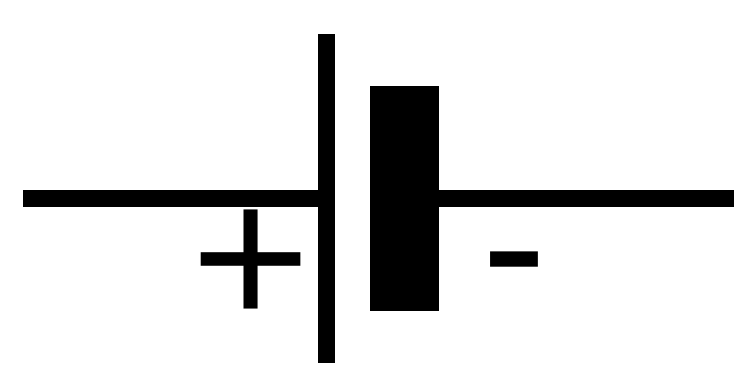
\includegraphics[scale=0.1]{./img/pile}	
			}
		\item Sur la pile plate la borne $[+]$ est la petite languette et la borne $[-]$ est la grande languette. Sur la pile rond, la borne $[+]$ se trouve sur le dessus et la borne $[-]$ sur le dessous.
		
		\item La valeur inscrite sur la pile plate est \num{4.5} $V$. Celle de la pile ronde est \num{1.5} $V$.
		\item L'unité de tension est le volt, son symbole est le $V$.
		\item Schéma électrique correspondant au montage :\\ 
		\begin{center}
			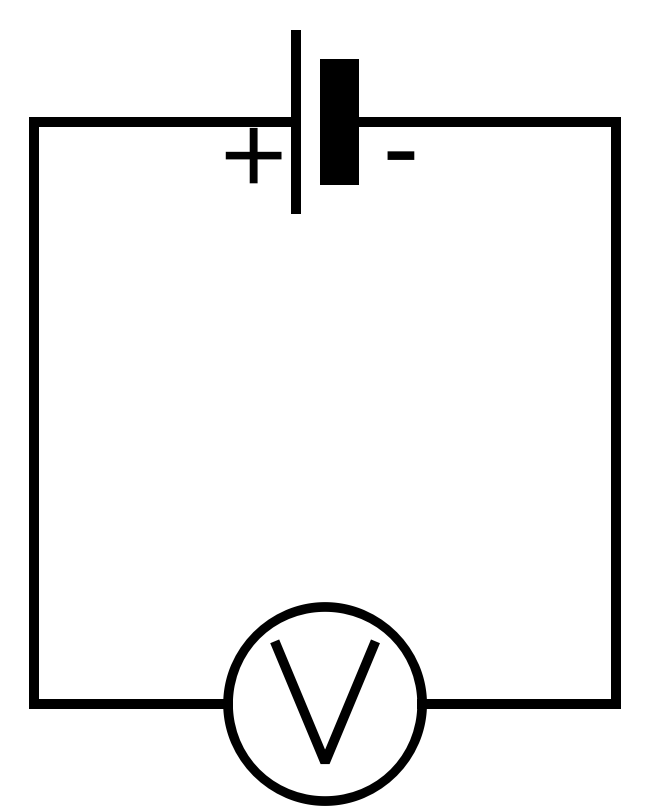
\includegraphics[scale=0.15]{img/pile_volt}
		\end{center}		
		
		\item Lorsque l'on inverse le branchement des bornes de la pile, on observe que la tension mesurée est négative.
		\item Pour mesurer une tension positive, la borne rouge du voltmètre doit être reliée à la borne positive de la pile.
	\end{enumerate}
\end{myact}

\begin{mybilan}
	L'unité de mesure de la tension électrique est le \kw{volt} (symbole $V$). Elle se mesure avec un \kw{voltmètre}.
	Pour mesurer la tension électrique d'une pile, on relie la \kw{borne rouge} du voltmètre à la \kw{borne $[+]$} de la pile et l'autre borne du voltmètre à la borne $[-]$.
\end{mybilan}

\begin{myexos}
	\twoCol{
	\begin{itemize}
		\item \exo{5}{97}
		\item \exo{6}{97}
		\item \exo{7}{97}
		\item \exo{15}{98}
	\end{itemize}}
\end{myexos}

\section{Mesure de tension électrique dans un circuit}

\begin{myrap}
	Un \kw{dipôle} est un composant électrique qui possède deux bornes (piles, lampes, interrupteurs, etc .).
\end{myrap}

\begin{myact}{3 page 92}
	\begin{enumerate}
		\item Un voltmètre se branche en dérivation aux bornes d'un dipôle.
		\item La tension aux bornes de la pile est plus faible lorsque le circuit est fermé.
		\item Lorsqu'elle n'est pas traversée par le courant, la tension aux bornes de la lampe est nulle.
		\item La tension aux bornes de l'interrupteur lorsqu'il est de \num{4.82} $V$. Lorsqu'il est fermé, elle est de \num{0} $V$.
		\item La tension aux bornes d'un fil de connexion est nulle.
	\end{enumerate}
\end{myact}

\begin{mybilan}
	Pour mesurer la tension aux bornes d'un dipôle placé dans un circuit, on branche un \kw{voltmètre en dérivation} entre les bornes de ce dipôle. Il existe une \kw{tension électrique} entre les bornes d'un \kw{interrupteur ouvert} placé dans un circuit.
	La tension électrique entre les bornes d'un fil de connexion est nulle.
\end{mybilan}

\begin{myexos}
	\begin{multicols}{2}
	
		\begin{itemize}
			\item \exo{8}{97}
			\item \exo{17}{98}
			
		\end{itemize}
	
	\end{multicols}
\end{myexos}

\section{Adaptation d'un dipôle}

\begin{myact}{4 page 93}
	\begin{enumerate}
		\item Pour vérifier que la lampe n'est pas grillée, on peut la brancher sur le générateur. \\
		\begin{center}
			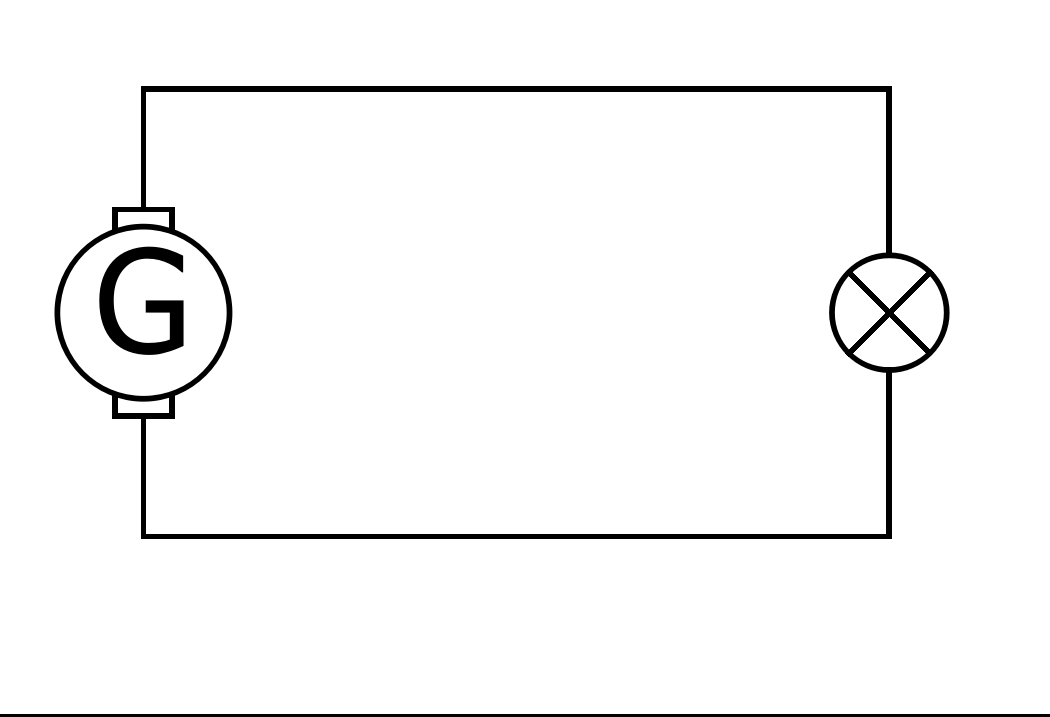
\includegraphics[scale=0.2]{img/gen_lamp}
		\end{center}
	
		\item On peut utiliser un voltmètre pour s'assurer que la pile est en bon état. Si la tension mesurée est proche de \num{1.5} $V$ alors la pile est en bon état.
		
		\item Pour obtenir différents éclats de la lampe, on fait varier la tension fournie par le générateur.
		
		\item On place un voltmètre aux bornes de la lampe lorsque l'on utilise le générateur, car on souhaite mesurer la tension du courant qui passe dans la lampe.
		
		\item \setlength{\tabcolsep}{4pt}
		\begin{tabular}{|l|c|c|c|c|c|c|}
			\hline
			Tension (en $V$)    & 3      & \num{4.5} & \num{6} & \num{7.5} & \num{9} & \num{12} \\ \hline
			\'Eclat de la lampe & éteinte & éteinte    & faible  & faible    & faible  & normal  \\ \hline
		\end{tabular}
	
		\item La condition de bon fonctionnement d'une lampe est que la tension à ses bornes doit être proche de la tension nominale.
	\end{enumerate}
\end{myact}

\begin{mybilan}
	La \kw{tension nominale} notée sur un appareil électrique est une indication de fonctionnement correct.
	Si la tension électrique aux bornes d'un dipôle est \kw{proche de sa tension nominale}, alors il y a \kw{adaptation} du dipôle au générateur. 
	Il y a \kw{sous-tension} si la tension est inférieure à la tension nominale. Il y a \kw{surtension} si elle est supérieure, le dipôle risque d'être détérioré. 
\end{mybilan}

\begin{myex}
	\twoCol{
		\begin{itemize}
			\item \exo{14}{98}
			\item \exo{18}{99}
			\item \exo{20}{99}
		\end{itemize}
	}
\end{myex}
\appendix

\newpage

\section*{Correction des exercices}

\subsection*{\exo{5}{97}}

\twoCol{
\begin{itemize}
	\item 1 $mV$ $=$ \textbf{\num{0.001}} $V$
	\item 1 $V$ $=$ \textbf{\num{1000}} $mV$
	\item 1 $kV$ $=$ \textbf{\num{1000}} $V$
	\item 1 $V$ $=$ \textbf{\num{0.001}} $kV$
	\item 1 $kV$ $=$ \textbf{\num{1000000}} $mV$
\end{itemize}}

\subsection*{\exo{6}{97}}


	\begin{enumerate}
		\item Incorrect : la borne COM du voltmètre doit être reliée à la borne négative $(-)$ du générateur.
		\item Incorrect : la borne rouge du voltmètre doit être reliée à la borne positive $(+)$ du générateur.
		\item Le montage est correct.
	\end{enumerate}


\subsection*{\exo{7}{97}}
\begin{multicols}{2}
	\begin{enumerate}
		\item 
	\end{enumerate}
\end{multicols}

\subsection*{\exo{8}{97}}


	\begin{enumerate}[label=\alph*)]
		\item 
	\end{enumerate}

\subsection*{\exo{14}{98}}

\subsection*{\exo{15}{98}}

\subsection*{\exo{17}{98}}

\subsection*{\exo{18}{99}}

\subsection*{\exo{20}{99}}
\end{document}]